\documentclass[11pt,a4paper]{article}

\usepackage[T1]{fontenc}
\usepackage[utf8]{inputenc}
\usepackage{lmodern}
\usepackage[margin=2.1cm,headheight=22pt]{geometry}
\usepackage[table]{xcolor}
\usepackage{amsmath,amssymb,mathtools}
\usepackage{booktabs,tabularx,array,multirow}
\usepackage{enumitem}
\usepackage{listings}
\usepackage{tikz}
\usetikzlibrary{arrows.meta,positioning,calc,fit}
\usepackage[most]{tcolorbox}
\usepackage{fancyhdr}
\usepackage{microtype}
\usepackage{hyperref}
\usepackage{url}

% ---------------------------------------------------------------------------
% Routly visual system
% ---------------------------------------------------------------------------
\definecolor{RoutlyNavy}{RGB}{27,38,79}
\definecolor{RoutlyBlue}{RGB}{56,85,163}
\definecolor{RoutlyOrange}{RGB}{237,152,42}
\definecolor{RoutlyTeal}{RGB}{0,150,136}
\definecolor{RoutlyRed}{RGB}{190,55,65}
\definecolor{RoutlyInk}{RGB}{32,36,45}
\definecolor{RoutlyMuted}{RGB}{102,112,132}
\definecolor{RoutlyLine}{RGB}{213,218,228}
\definecolor{RoutlyPaper}{RGB}{247,248,251}
\definecolor{PNPColor}{RGB}{27,38,79}
\definecolor{CNPColor}{RGB}{222,139,30}
\definecolor{CNCColor}{RGB}{0,137,123}
\definecolor{CLPColor}{RGB}{56,85,163}
\definecolor{CLCColor}{RGB}{190,55,65}

\hypersetup{
  colorlinks=true,
  linkcolor=RoutlyBlue,
  urlcolor=RoutlyBlue,
  pdftitle={Where the Grounding Formulae Come From},
  pdfauthor={Routly},
  pdfsubject={Formula-to-PDDL guide for model-side scalability}
}

\setlength{\parindent}{0pt}
\setlength{\parskip}{0.55em}
\setlist[itemize]{leftmargin=1.45em,itemsep=0.25em,topsep=0.25em}
\setlist[enumerate]{leftmargin=1.65em,itemsep=0.25em,topsep=0.25em}
\renewcommand{\arraystretch}{1.18}

\pagestyle{fancy}
\fancyhf{}
\fancyhead[L]{\small\textcolor{RoutlyNavy}{\textbf{Routly}}}
\fancyhead[R]{\small\textcolor{RoutlyMuted}{Grounding formulae}}
\fancyfoot[L]{\small\textcolor{RoutlyMuted}{Model-side scalability technical reference}}
\fancyfoot[R]{\small\textcolor{RoutlyNavy}{\thepage}}
\renewcommand{\headrulewidth}{0.4pt}
\renewcommand{\headrule}{\hbox to\headwidth{\color{RoutlyLine}\leaders\hrule height \headrulewidth\hfill}}
\renewcommand{\footrulewidth}{0pt}

\newcolumntype{Y}{>{\raggedright\arraybackslash}X}
\newcolumntype{C}[1]{>{\centering\arraybackslash}p{#1}}

\makeatletter
\renewcommand{\section}{\@startsection{section}{1}{0pt}
  {-2.2ex plus -0.5ex minus -0.2ex}
  {1.0ex plus 0.2ex}
  {\normalfont\Large\bfseries\color{RoutlyNavy}}}
\renewcommand{\subsection}{\@startsection{subsection}{2}{0pt}
  {-1.8ex plus -0.4ex minus -0.2ex}
  {0.75ex plus 0.2ex}
  {\normalfont\large\bfseries\color{RoutlyNavy}}}
\renewcommand{\subsubsection}{\@startsection{subsubsection}{3}{0pt}
  {-1.4ex plus -0.3ex minus -0.2ex}
  {0.55ex plus 0.1ex}
  {\normalfont\normalsize\bfseries\color{RoutlyBlue}}}
\makeatother

\newtcolorbox{keybox}[1][]{
  enhanced,
  breakable,
  colback=RoutlyOrange!8,
  colframe=RoutlyOrange,
  boxrule=0.8pt,
  arc=2mm,
  left=2.5mm,right=2.5mm,top=2mm,bottom=2mm,
  fonttitle=\bfseries\color{RoutlyNavy},
  title={Key point},
  #1
}

\newtcolorbox{definitionbox}[1][]{
  enhanced,
  breakable,
  colback=RoutlyBlue!5,
  colframe=RoutlyBlue!65,
  boxrule=0.7pt,
  arc=2mm,
  left=2.5mm,right=2.5mm,top=2mm,bottom=2mm,
  #1
}

\newtcolorbox{defencebox}[1][]{
  enhanced,
  breakable,
  colback=RoutlyTeal!6,
  colframe=RoutlyTeal,
  boxrule=0.8pt,
  arc=2mm,
  left=2.5mm,right=2.5mm,top=2mm,bottom=2mm,
  fonttitle=\bfseries\color{RoutlyNavy},
  title={Interpretation},
  #1
}

\newtcolorbox{warningbox}[1][]{
  enhanced,
  breakable,
  colback=RoutlyRed!5,
  colframe=RoutlyRed!80,
  boxrule=0.7pt,
  arc=2mm,
  left=2.5mm,right=2.5mm,top=2mm,bottom=2mm,
  #1
}

\newcommand{\configbanner}[4]{%
  \begin{tcolorbox}[
    enhanced,
    colback=#1!8,
    colframe=#1,
    boxrule=0.9pt,
    arc=2mm,
    left=3mm,right=3mm,top=2.5mm,bottom=2.5mm]
    {\LARGE\bfseries\textcolor{#1}{#2}}\hfill
    {\large\bfseries\textcolor{RoutlyNavy}{#3}}\\[1mm]
    {\small\textcolor{RoutlyInk}{#4}}
  \end{tcolorbox}
}

\newcommand{\formularesult}[3]{%
  \begin{tcolorbox}[
    enhanced,
    colback=#1!5,
    colframe=#1!80,
    boxrule=0.8pt,
    arc=2mm,
    left=2.5mm,right=2.5mm,top=2mm,bottom=2mm]
    \centering
    {\small\bfseries\textcolor{RoutlyMuted}{COMPACT SLIDE FORMULA}}\\[1mm]
    {\Large\bfseries\boldmath \(#2\)}\\[1mm]
    {\normalsize #3}
  \end{tcolorbox}
}

\lstdefinelanguage{PDDL}{
  morekeywords={
    define,domain,requirements,types,predicates,functions,objects,init,goal,
    action,process,event,parameters,precondition,effect,and,not,assign,
    increase,decrease,at,road-open,connects,static-road,dynamic-road,
    current-window,next-window,ready-road,road-next,goal-road,moving,on-road,
    reached-goal,vehicle,road,location,time-window
  },
  sensitive=true,
  morecomment=[l]{;;},
  morestring=[b]"
}

\lstset{
  language=PDDL,
  basicstyle=\ttfamily\scriptsize,
  keywordstyle=\color{RoutlyBlue}\bfseries,
  commentstyle=\color{RoutlyMuted}\itshape,
  stringstyle=\color{RoutlyRed},
  showstringspaces=false,
  columns=fullflexible,
  keepspaces=true,
  breaklines=true,
  breakatwhitespace=true,
  frame=single,
  framerule=0.4pt,
  rulecolor=\color{RoutlyLine},
  backgroundcolor=\color{RoutlyPaper},
  xleftmargin=1.5mm,
  xrightmargin=1.5mm,
  aboveskip=0.6em,
  belowskip=0.6em,
  tabsize=2
}

\newcommand{\codeorigin}[1]{%
  {\footnotesize\textcolor{RoutlyMuted}{Generator origin: \texttt{#1}}\par}
}

\begin{document}

% ---------------------------------------------------------------------------
% Cover
% ---------------------------------------------------------------------------
\thispagestyle{empty}
\begin{tikzpicture}[remember picture,overlay]
  \fill[RoutlyNavy] (current page.south west) rectangle (current page.north east);
  \fill[RoutlyOrange]
    ([yshift=-5.25cm]current page.north west)
    rectangle
    ([yshift=-5.10cm]current page.north east);
  \fill[RoutlyBlue!35]
    ([xshift=-2.0cm,yshift=1.6cm]current page.south east)
    circle (4.1cm);
  \fill[RoutlyNavy]
    ([xshift=-2.0cm,yshift=1.6cm]current page.south east)
    circle (3.65cm);
\end{tikzpicture}

\vspace*{1.35cm}
{\color{RoutlyOrange}\Large\bfseries RQ1 TECHNICAL REFERENCE\par}
\vspace{1.65cm}
{\color{white}\fontsize{30}{34}\selectfont\bfseries
Where the Grounding\\Formulae Come From\par}
\vspace{0.65cm}
{\color{white!82}\Large
A formula-to-PDDL guide for Routly's five\\model-side configurations\par}
\vspace{1.2cm}
\begin{tcolorbox}[
  width=0.83\textwidth,
  colback=RoutlyBlue!18!RoutlyNavy,
  colframe=white!45,
  boxrule=0.7pt,
  arc=2mm,
  left=4mm,right=4mm,top=3mm,bottom=3mm]
  \color{white}
  \textbf{Reference case:} 500 requested nodes, hybrid congestion,
  after macro-road preprocessing.\\
  \textbf{Purpose:} explain every term shown on presentation slide 16,
  connect it to the generated PDDL, and clarify what the formula can and
  cannot say about runtime.
\end{tcolorbox}
\vfill
{\color{white!65}\large Routly --- Hybrid Planning for Urban Routing\par}
\newpage

\begingroup
\small
\setcounter{tocdepth}{1}
\tableofcontents
\endgroup
\newpage

% ---------------------------------------------------------------------------
\section{How to read slide 16}

\begin{keybox}
Slide 16 is \textbf{not a direct runtime predictor}. It separates two
quantities that contribute to grounding in different ways:
\textbf{candidate exposure} and \textbf{retained grounded structures}.
\end{keybox}

\begin{definitionbox}
\textbf{Candidates} is a deliberately loose, type-based Cartesian upper
bound. It counts assignments that are compatible with the declared PDDL
types before static predicates such as \texttt{connects},
\texttt{road-next}, \texttt{static-road}, \texttt{goal-road}, and
\texttt{next-window} remove impossible combinations.

\textbf{Retained (derived)} is the number of valid grounded mechanisms left
after static filtering. These are not the actions executed in the final plan.
They are the actions, events, and processes made available to the subsequent
search.
\end{definitionbox}

\subsection{The two-stage interpretation}

\begin{center}
{\small\bfseries\color{RoutlyOrange}
Static predicates filter the topology\par}
\vspace{1mm}
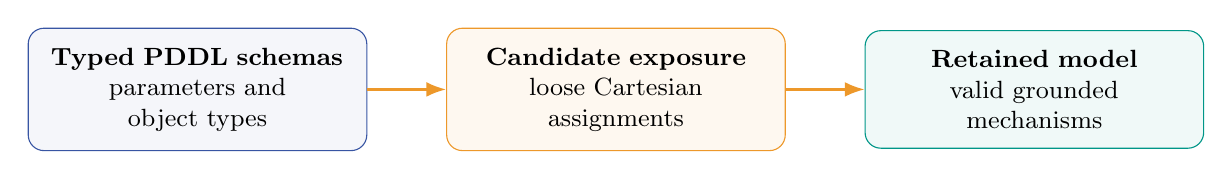
\begin{tikzpicture}[
  node distance=8mm and 10mm,
  box/.style={
    draw,rounded corners=2mm,align=center,
    minimum height=12mm,text width=3.8cm,
    inner sep=2.5mm,font=\small
  },
  arr/.style={-{Latex[length=2.5mm]},thick,RoutlyOrange}
]
  \node[box,draw=RoutlyBlue,fill=RoutlyBlue!5] (types)
    {\textbf{Typed PDDL schemas}\\parameters and object types};
  \node[box,draw=RoutlyOrange,fill=RoutlyOrange!7,right=of types] (cand)
    {\textbf{Candidate exposure}\\loose Cartesian assignments};
  \node[box,draw=RoutlyTeal,fill=RoutlyTeal!6,right=of cand] (ret)
    {\textbf{Retained model}\\valid grounded mechanisms};
  \draw[arr] (types) -- (cand);
  \draw[arr] (cand) -- (ret);
\end{tikzpicture}
\end{center}

Candidate exposure describes the potential cost of \emph{reaching} the valid
model. Retained structures describe the cost of materialising, storing, and
preprocessing the valid model that remains. The two quantities are related,
but they are not added linearly and neither one alone predicts elapsed time.

\subsection{Reference-case notation}

\begin{table}[h]
\centering
\caption{Symbols used throughout the derivations.}
\begin{tabularx}{\textwidth}{@{}C{1.45cm}C{1.8cm}@{\hspace{0.8em}}Y@{}}
\toprule
\textbf{Symbol} & \textbf{Value} & \textbf{Meaning}\\
\midrule
\(R\)   & \(829\)   & Road objects after macro-road preprocessing.\\
\(L\)   & \(483\)   & Location objects after macro-road preprocessing.\\
\(W\)   & \(21\)    & Global congestion windows.\\
\(S\)   & \(782\)   & Roads selected as static by hybrid congestion.\\
\(D\)   & \(47\)    & Roads retained as dynamic; \(S+D=R\).\\
\(T_s\) & \(1{,}471\) & Valid line-graph transitions whose current road is static.\\
\(T_d\) & \(79\)    & Valid line-graph transitions whose current road is dynamic.\\
\(A\)   & --- & Retained action.\\
\(E\)   & --- & Retained event.\\
\(P\)   & --- & Retained process.\\
\bottomrule
\end{tabularx}
\end{table}

The experiment contains one vehicle. A vehicle factor would therefore be
\(V=1\), so it is omitted from all slide formulae.

\subsection{Three reusable counting rules}

\begin{enumerate}
  \item A schema with parameters
  \texttt{?r - road ?from - location ?to - location}
  exposes \(R L^2\) typed assignments before \texttt{connects} is evaluated.

  \item A static schema contributes one copy of the topology product. A
  dynamic schema with parameter \texttt{?w - time-window} contributes \(W\)
  copies. Together they produce the multiplier \(1+W\).

  \item The event below has two window parameters. Its loose exposure is
  \(W^2\), but the static chain \texttt{next-window} retains only adjacent
  pairs, hence \(W-1=20\) events.
\end{enumerate}

\begin{lstlisting}
(:event advance-window
 :parameters (?from - time-window ?to - time-window)
 :precondition (and
   (current-window ?from)
   (next-window ?from ?to)
   (>= (sim-time) (window-start ?to)))
 :effect (and
   (not (current-window ?from))
   (current-window ?to)))
\end{lstlisting}
\codeorigin{src/routly/pddl/domain\_generator.py :: \_build\_events}

\[
\underbrace{W^2}_{21^2=441\ \text{candidates}}
\quad\xrightarrow{\texttt{next-window}}\quad
\underbrace{W-1}_{20\ \text{retained events}}.
\]

% ---------------------------------------------------------------------------
\section{PNP: process, node-based, parameterized}

\configbanner{PNPColor}{PNP}{Process + node-based + parameterized}{
The expressive baseline: ENHSP receives generic road/location schemas and
represents the vehicle while it is travelling along a road.}

\formularesult{PNPColor}
  {R L^2(W+3)+W^2+1}
  {\(=4{,}641{,}518{,}386\approx4.642\times10^9\) candidates}

\subsection{Expanded derivation}

\[
\boxed{
\underbrace{R L^2(1+W)}_{\text{start actions}}
+
\underbrace{2R L^2}_{\text{arrival events}}
+
\underbrace{W^2}_{\text{advance-window event}}
+
\underbrace{1}_{\text{continuous process}}
}
\]

The compact term \(W+3\) is simply:
\[
W+3=(1+W)+2.
\]

\begin{table}[h]
\centering
\caption{PNP candidate terms and their PDDL origin.}
\begin{tabularx}{\textwidth}{@{}C{3.0cm}Y C{3.0cm}@{}}
\toprule
\textbf{Term} & \textbf{Origin} & \textbf{Reference value}\\
\midrule
\(R L^2\) &
Static \texttt{start-traversal-static}: road, origin, destination. &
\(193{,}396{,}581\)\\
\addlinespace[2pt]
\(R L^2W\) &
Dynamic \texttt{start-traversal-dynamic}: the same parameters plus a window. &
\(4{,}061{,}328{,}201\)\\
\addlinespace[2pt]
\(2R L^2\) &
Two generic arrival schemas: normal intersection and traffic-light intersection. &
\(386{,}793{,}162\)\\
\addlinespace[2pt]
\(W^2\) &
\texttt{advance-window} binds a from-window and a to-window. &
\(441\)\\
\addlinespace[2pt]
\(1\) &
\texttt{traverse} has only one vehicle parameter and \(V=1\). &
\(1\)\\
\bottomrule
\end{tabularx}
\end{table}

\subsection{PDDL correspondence}

\begin{lstlisting}
(:action start-traversal-static
 :parameters (?v - vehicle ?r - road
              ?from - location ?to - location)
 :precondition (and
   (at ?v ?from) (connects ?r ?from ?to)
   (road-open ?r) (static-road ?r) (not (moving ?v)))
 :effect (and
   (not (at ?v ?from)) (on-road ?v ?r) (moving ?v)
   (assign (distance-remaining ?v) (road-length ?r))))

(:action start-traversal-dynamic
 :parameters (?v - vehicle ?r - road
              ?from - location ?to - location
              ?w - time-window)
 :precondition (and
   (at ?v ?from) (connects ?r ?from ?to)
   (road-open ?r) (dynamic-road ?r) (current-window ?w)
   (not (moving ?v)))
 :effect (and
   (not (at ?v ?from)) (on-road ?v ?r) (moving ?v)
   (assign (distance-remaining ?v) (road-length ?r))))
\end{lstlisting}
\codeorigin{src/routly/pddl/domain\_generator.py :: \_build\_process\_start\_action}

\begin{lstlisting}
(:process traverse
 :parameters (?v - vehicle)
 :precondition (and
   (moving ?v) (> (distance-remaining ?v) 0))
 :effect (and
   (decrease (distance-remaining ?v) (* #t (speed ?v)))
   (increase (total-distance ?v) (* #t (speed ?v)))
   (increase (sim-time) (* #t 1))))
\end{lstlisting}
\codeorigin{src/routly/pddl/domain\_generator.py :: \_build\_process}

\begin{lstlisting}
(:event arrive
 :parameters (?v - vehicle ?r - road
              ?from - location ?to - location)
 :precondition (and
   (on-road ?v ?r) (moving ?v)
   (connects ?r ?from ?to)
   (not (has-traffic-light ?to))
   (<= (distance-remaining ?v) 0))
 :effect (and
   (not (on-road ?v ?r)) (not (moving ?v)) (at ?v ?to)))

(:event arrive-at-traffic-light
 :parameters (?v - vehicle ?r - road
              ?from - location ?to - location)
 :precondition (and
   (on-road ?v ?r) (moving ?v)
   (connects ?r ?from ?to)
   (has-traffic-light ?to)
   (<= (distance-remaining ?v) 0))
 :effect (and
   (not (on-road ?v ?r)) (not (moving ?v)) (at ?v ?to)
   (increase (travel-time ?v) (light-wait ?to))))
\end{lstlisting}
\codeorigin{src/routly/pddl/domain\_generator.py :: \_build\_events}

\subsection{From candidates to retained structures}

Static predicates select the real topology:
\[
\underbrace{S+DW}_{782+47\cdot21=1{,}769\ A}
\]
\[
\underbrace{R}_{829\ \text{arrival events}}
+
\underbrace{(W-1)}_{20\ \text{window events}}
=849E.
\]
There is one vehicle process:
\[
\boxed{1{,}769A+849E+1P=2{,}619\ \text{retained mechanisms}.}
\]

Although two arrival schemas exist, each real road ends either at a
signalised node or at a non-signalised node. Static filtering therefore
retains one arrival event per road, not two.

\begin{defencebox}
PNP is large for two independent reasons: the generic node-based schemas
expose the \(R L^2\) Cartesian product, and the process semantics retain
arrival events plus a continuous process in the final grounded model.
\end{defencebox}

% ---------------------------------------------------------------------------
\section{CNP: compiled duration, node-based, parameterized}

\configbanner{CNPColor}{CNP}{Compiled duration + node-based + parameterized}{
The traversal semantics are compiled into one numeric action, but ENHSP still
receives generic road/from/to parameters.}

\formularesult{CNPColor}
  {R L^2(1+W)+W^2}
  {\(=4{,}254{,}725{,}223\approx4.255\times10^9\) candidates}

\subsection{What disappears relative to PNP}

\[
\begin{aligned}
\text{PNP}
&=\underbrace{R L^2(1+W)}_{\text{start actions}}
 +\underbrace{2R L^2}_{\text{arrival events}}
 +\underbrace{W^2}_{\text{window event}}
 +\underbrace{1}_{\text{process}},\\
\text{CNP}
&=\underbrace{R L^2(1+W)}_{\text{compiled traversal actions}}
 +\underbrace{W^2}_{\text{window event}}.
\end{aligned}
\]

Compiled duration removes the two generic arrival-event schemas and the
continuous process. It does \emph{not} remove the dominant road/from/to
Cartesian product because action generation remains parameterized.

\subsection{PDDL correspondence}

\begin{lstlisting}
(:action traverse-road-static
 :parameters (?v - vehicle ?r - road
              ?from - location ?to - location)
 :precondition (and
   (at ?v ?from) (connects ?r ?from ?to)
   (road-open ?r) (static-road ?r))
 :effect (and
   (not (at ?v ?from)) (at ?v ?to)
   (increase (travel-time ?v) (travel-duration ?r))
   (increase (sim-time) (travel-duration ?r))))

(:action traverse-road-dynamic
 :parameters (?v - vehicle ?r - road
              ?from - location ?to - location
              ?w - time-window)
 :precondition (and
   (at ?v ?from) (connects ?r ?from ?to)
   (road-open ?r) (dynamic-road ?r) (current-window ?w))
 :effect (and
   (not (at ?v ?from)) (at ?v ?to)
   (increase (travel-time ?v) (travel-duration-window ?r ?w))
   (increase (sim-time) (travel-duration-window ?r ?w))))
\end{lstlisting}
\codeorigin{src/routly/pddl/domain\_generator.py :: \_build\_compiled\_duration\_action}

There is no hidden process maintaining time. The action directly increases
\texttt{sim-time}. Once it crosses the start of the next window, the generic
\texttt{advance-window} event becomes applicable.

\subsection{Numeric derivation}

\[
\begin{aligned}
R L^2(1+W)
&=829\cdot483^2\cdot22\\
&=4{,}254{,}724{,}782,\\
W^2&=21^2=441,\\
\text{total}
&=4{,}254{,}725{,}223.
\end{aligned}
\]

After static filtering:
\[
\boxed{1{,}769A+20E=1{,}789\ \text{retained mechanisms}.}
\]

\begin{defencebox}
CNP is structurally lighter than PNP because compiled duration removes the
arrival events and the process. However, its candidate exposure remains in the
same order of magnitude because \texttt{?r}, \texttt{?from}, and \texttt{?to}
are still generic.
\end{defencebox}

% ---------------------------------------------------------------------------
\section{CNC: compiled duration, node-based, compiled}

\configbanner{CNCColor}{CNC}{Compiled duration + node-based + compiled}{
Python instantiates the valid road/end-point combinations and uses singleton
types so that each specialised parameter has exactly one compatible object.}

\formularesult{CNCColor}
  {S+DW+W^2}
  {\(=2{,}210\) candidates}

\subsection{From a generic action to one specialised schema}

\begin{center}
{\small\bfseries\color{RoutlyOrange}
Same retained model, different candidate exposure\par}
\vspace{1mm}
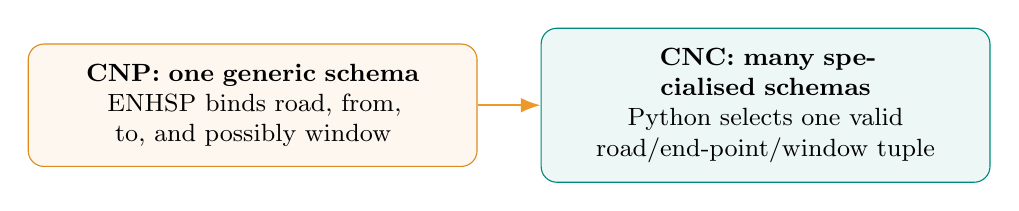
\begin{tikzpicture}[
  node distance=8mm,
  box/.style={
    draw,rounded corners=2mm,align=center,
    text width=5.2cm,minimum height=13mm,
    inner sep=2.5mm,font=\small
  },
  arr/.style={-{Latex[length=2.5mm]},thick,RoutlyOrange}
]
  \node[box,draw=CNPColor,fill=CNPColor!7] (generic)
    {\textbf{CNP: one generic schema}\\
     ENHSP binds road, from, to, and possibly window};
  \node[box,draw=CNCColor,fill=CNCColor!7,right=of generic] (compiled)
    {\textbf{CNC: many specialised schemas}\\
     Python selects one valid road/end-point/window tuple};
  \draw[arr] (generic) -- (compiled);
\end{tikzpicture}
\end{center}

\begin{lstlisting}
(:types
  vehicle location road time-window - object
  loc_type_loc_a loc_type_loc_b - location
  road_type_road_0001 - road
  window_type_tw_00000 - time-window)

(:objects
  vehicle_0 - vehicle
  loc_a - loc_type_loc_a
  loc_b - loc_type_loc_b
  road_0001 - road_type_road_0001
  tw_00000 - window_type_tw_00000)
\end{lstlisting}
\codeorigin{domain\_generator.py :: \_build\_types;\\
problem\_generator.py :: \_build\_objects}

\begin{lstlisting}
(:action traverse-road-dynamic-road_0001-tw_00000
 :parameters (?v - vehicle
              ?r - road_type_road_0001
              ?from - loc_type_loc_a
              ?to - loc_type_loc_b
              ?w - window_type_tw_00000)
 :precondition (and
   (at ?v ?from) (connects ?r ?from ?to)
   (road-open ?r) (dynamic-road ?r) (current-window ?w))
 :effect (and
   (not (at ?v ?from)) (at ?v ?to)
   (increase (travel-time ?v) (travel-duration-window ?r ?w))
   (increase (sim-time) (travel-duration-window ?r ?w))))
\end{lstlisting}
\codeorigin{src/routly/pddl/domain\_generator.py :: \_build\_compiled\_duration\_road\_actions}

The action still has normal PDDL parameters. The difference is that every
specialised type contains one object, so this schema exposes one legal binding
instead of a generic Cartesian product.

\subsection{Candidate derivation}

\[
\underbrace{S}_{\substack{\text{one specialised schema}\\\text{per static road}}}
+
\underbrace{DW}_{\substack{\text{one specialised schema}\\
\text{per dynamic road/window}}}
+
\underbrace{W^2}_{\text{generic advance-window}}
\]
\[
782+(47\cdot21)+21^2
=782+987+441
=\boxed{2{,}210}.
\]

The first two terms are already valid by construction. Only
\texttt{advance-window} remains generic:
\[
\boxed{1{,}769A+20E=1{,}789\ \text{retained mechanisms}.}
\]

\begin{keybox}
CNP and CNC retain the same final model: \(1{,}769A+20E\). The difference is
the path used to reach it. CNP exposes roughly \(4.255\) billion typed
assignments; CNC exposes \(2{,}210\).
\end{keybox}

\begin{defencebox}
This is the cleanest evidence for singleton types. They do not change which
movements are available after grounding; they move the valid instantiation
from ENHSP to Python and collapse the generic binding space.
\end{defencebox}

% ---------------------------------------------------------------------------
\section{CLP: compiled duration, line graph, parameterized}

\configbanner{CLPColor}{CLP}{Compiled duration + line graph + parameterized}{
The vehicle state is attached to the current road. A generic action chooses
the current road and a possible successor road.}

\formularesult{CLPColor}
  {R(R+1)(1+W)+W^2}
  {\(=15{,}137{,}981\approx1.514\times10^7\) candidates}

\subsection{Expanded derivation}

\[
\boxed{
\underbrace{R^2(1+W)}_{\text{road-to-road traversal}}
+
\underbrace{R(1+W)}_{\text{finish-road}}
+
\underbrace{W^2}_{\text{advance-window}}
}
\]
\[
R^2(1+W)+R(1+W)
=R(R+1)(1+W).
\]

\begin{table}[h]
\centering
\caption{CLP candidate terms and their PDDL origin.}
\begin{tabularx}{\textwidth}{@{}C{3.1cm}Y@{}}
\toprule
\textbf{Term} & \textbf{Origin}\\
\midrule
\(R^2\) &
\texttt{traverse-road-static} binds a current road and a possible next road.\\
\addlinespace[3pt]
\(R^2W\) &
\texttt{traverse-road-dynamic} adds a window parameter.\\
\addlinespace[3pt]
\(R\) &
\texttt{finish-road-static} binds only the current goal road candidate.\\
\addlinespace[3pt]
\(RW\) &
\texttt{finish-road-dynamic} adds a window parameter.\\
\addlinespace[3pt]
\(W^2\) &
The shared generic \texttt{advance-window} event.\\
\bottomrule
\end{tabularx}
\end{table}

\subsection{PDDL correspondence}

\begin{lstlisting}
(:action traverse-road-static
 :parameters (?v - vehicle ?r - road ?next - road)
 :precondition (and
   (ready-road ?v ?r) (road-next ?r ?next)
   (road-open ?r) (static-road ?r))
 :effect (and
   (not (ready-road ?v ?r)) (ready-road ?v ?next)
   (increase (travel-time ?v) (travel-duration ?r))
   (increase (sim-time) (travel-duration ?r))))

(:action traverse-road-dynamic
 :parameters (?v - vehicle ?r - road ?next - road
              ?w - time-window)
 :precondition (and
   (ready-road ?v ?r) (road-next ?r ?next)
   (road-open ?r) (dynamic-road ?r) (current-window ?w))
 :effect (and
   (not (ready-road ?v ?r)) (ready-road ?v ?next)
   (increase (travel-time ?v) (travel-duration-window ?r ?w))
   (increase (sim-time) (travel-duration-window ?r ?w))))
\end{lstlisting}
\codeorigin{src/routly/pddl/domain\_generator.py :: \_build\_compiled\_duration\_line\_graph\_action}

\begin{lstlisting}
(:action finish-road-static
 :parameters (?v - vehicle ?r - road)
 :precondition (and
   (ready-road ?v ?r) (goal-road ?r)
   (road-open ?r) (static-road ?r))
 :effect (and
   (not (ready-road ?v ?r)) (reached-goal ?v)
   (increase (travel-time ?v) (travel-duration ?r))
   (increase (sim-time) (travel-duration ?r))))

(:action finish-road-dynamic
 :parameters (?v - vehicle ?r - road ?w - time-window)
 :precondition (and
   (ready-road ?v ?r) (goal-road ?r)
   (road-open ?r) (dynamic-road ?r) (current-window ?w))
 :effect (and
   (not (ready-road ?v ?r)) (reached-goal ?v)
   (increase (travel-time ?v) (travel-duration-window ?r ?w))
   (increase (sim-time) (travel-duration-window ?r ?w))))
\end{lstlisting}
\codeorigin{src/routly/pddl/domain\_generator.py :: \_build\_compiled\_duration\_line\_graph\_action}

\subsection{Numeric derivation and static filtering}

\[
\begin{aligned}
R(R+1)(1+W)
&=829\cdot830\cdot22\\
&=15{,}137{,}540,\\
W^2&=441,\\
\text{total}&=15{,}137{,}981.
\end{aligned}
\]

The problem generator creates \texttt{road-next} only for true graph
successors:
\begin{lstlisting}
(road-next road_0001 road_0007)
(road-next road_0001 road_0012)
...
(goal-road road_goal)
\end{lstlisting}
\codeorigin{src/routly/pddl/problem\_generator.py :: \_build\_init}

After static filtering:
\[
\underbrace{T_s+T_dW}_{1{,}471+79\cdot21=3{,}130\ \text{traversals}}
+
\underbrace{1}_{\text{valid finish-road}}
+
\underbrace{20}_{\text{window events}}
=\boxed{3{,}151}.
\]

The selected goal road is static in this reference instance, so one finish
action is retained. If the selected goal road were dynamic, its retained
finish contribution would be \(W\) rather than \(1\).

\begin{defencebox}
The line graph reduces parameter arity and therefore candidate exposure.
However, it retains more actions than the node-based encoding because one
current road may have several valid successor roads.
\end{defencebox}

% ---------------------------------------------------------------------------
\section{CLC: compiled duration, line graph, compiled}

\configbanner{CLCColor}{CLC}{Compiled duration + line graph + compiled}{
Python enumerates only valid road-to-road transitions and assigns singleton
types to the current road, successor road, and, when required, window.}

\formularesult{CLCColor}
  {T_s+T_dW+1+W^2}
  {\(=3{,}572\) candidates}

\subsection{Specialised line-graph action}

\begin{lstlisting}
(:action traverse-road-dynamic-road_0001-road_0007-tw_00000
 :parameters (?v - vehicle
              ?r - road_type_road_0001
              ?next - road_type_road_0007
              ?w - window_type_tw_00000)
 :precondition (and
   (ready-road ?v ?r) (road-next ?r ?next)
   (road-open ?r) (dynamic-road ?r) (current-window ?w))
 :effect (and
   (not (ready-road ?v ?r)) (ready-road ?v ?next)
   (increase (travel-time ?v) (travel-duration-window ?r ?w))
   (increase (sim-time) (travel-duration-window ?r ?w))))
\end{lstlisting}
\codeorigin{domain\_generator.py ::\\
\_build\_compiled\_duration\_line\_graph\_road\_actions}

\begin{lstlisting}
(:action finish-road-static-road_goal
 :parameters (?v - vehicle ?r - road_type_road_goal)
 :precondition (and
   (ready-road ?v ?r) (goal-road ?r)
   (road-open ?r) (static-road ?r))
 :effect (and
   (not (ready-road ?v ?r)) (reached-goal ?v)
   (increase (travel-time ?v) (travel-duration ?r))
   (increase (sim-time) (travel-duration ?r))))
\end{lstlisting}
\codeorigin{domain\_generator.py ::\\
\_build\_compiled\_duration\_line\_graph\_road\_actions}

\subsection{Candidate derivation}

\[
\underbrace{T_s}_{\text{static valid transitions}}
+
\underbrace{T_dW}_{\text{dynamic valid transition/window pairs}}
+
\underbrace{1}_{\text{static goal-road finish}}
+
\underbrace{W^2}_{\text{generic window event}}.
\]
\[
1{,}471+(79\cdot21)+1+441
=1{,}471+1{,}659+1+441
=\boxed{3{,}572}.
\]

After \texttt{next-window} filtering:
\[
\boxed{3{,}130\ \text{traversal actions}
+1\ \text{finish action}
+20\ \text{events}
=3{,}151.}
\]

\begin{center}
{\small\bfseries\color{RoutlyOrange}
Same retained model, different candidate exposure\par}
\vspace{1mm}
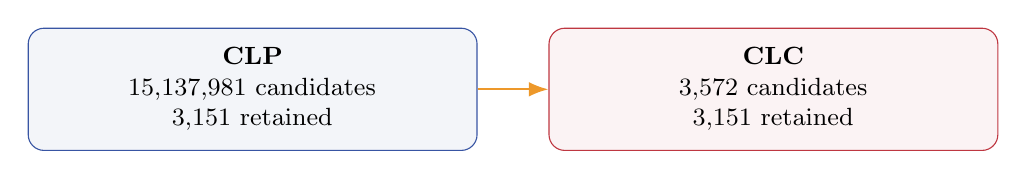
\begin{tikzpicture}[
  node distance=9mm,
  box/.style={
    draw,rounded corners=2mm,align=center,
    text width=5.2cm,minimum height=15mm,
    inner sep=2.5mm,font=\small
  },
  arr/.style={-{Latex[length=2.5mm]},thick,RoutlyOrange}
]
  \node[box,draw=CLPColor,fill=CLPColor!6] (clp)
    {\textbf{CLP}\\
     \(15{,}137{,}981\) candidates\\
     \(3{,}151\) retained};
  \node[box,draw=CLCColor,fill=CLCColor!6,right=of clp] (clc)
    {\textbf{CLC}\\
     \(3{,}572\) candidates\\
     \(3{,}151\) retained};
  \draw[arr] (clp) -- (clc);
\end{tikzpicture}
\end{center}

\begin{defencebox}
CLP and CLC retain the same grounded model. CLC is faster because singleton
types remove almost all generic binding exploration, not because it removes
valid line-graph transitions.
\end{defencebox}

% ---------------------------------------------------------------------------
\section{All five configurations side by side}

\begin{table}[h]
\centering
\caption{Complete 500-node hybrid reference-case decomposition.}
\small
\begin{tabularx}{\textwidth}{@{}C{1.0cm}Y C{2.6cm} C{2.5cm}@{}}
\toprule
\textbf{Code} & \textbf{Candidate formula} &
\textbf{Candidates} & \textbf{Retained}\\
\midrule
\textcolor{PNPColor}{\textbf{PNP}} &
\(RL^2(1+W)+2RL^2+W^2+1\) &
\(4.642\times10^9\) &
\(2{,}619\)\\
\textcolor{CNPColor}{\textbf{CNP}} &
\(RL^2(1+W)+W^2\) &
\(4.255\times10^9\) &
\(1{,}789\)\\
\textcolor{CNCColor}{\textbf{CNC}} &
\(S+DW+W^2\) &
\(2{,}210\) &
\(1{,}789\)\\
\textcolor{CLPColor}{\textbf{CLP}} &
\(R^2(1+W)+R(1+W)+W^2\) &
\(1.514\times10^7\) &
\(3{,}151\)\\
\textcolor{CLCColor}{\textbf{CLC}} &
\(T_s+T_dW+1+W^2\) &
\(3{,}572\) &
\(3{,}151\)\\
\bottomrule
\end{tabularx}
\end{table}

\subsection{What each modelling axis changes}

\begin{table}[h]
\centering
\begin{tabularx}{\textwidth}{@{}C{3.0cm}Y Y@{}}
\toprule
\textbf{Axis} & \textbf{Structural effect} & \textbf{Visible comparison}\\
\midrule
Traversal &
Compiled duration removes process and arrival-event semantics. &
PNP \(\rightarrow\) CNP\\
State &
Line graph replaces two location parameters with a current/next-road pair,
but may retain more transitions because of branching. &
CNP \(\leftrightarrow\) CLP\\
Generation &
Singleton types move valid instantiation from ENHSP to Python. &
CNP \(\rightarrow\) CNC; CLP \(\rightarrow\) CLC\\
\bottomrule
\end{tabularx}
\end{table}

\subsection{The two strongest controlled comparisons}

\begin{definitionbox}
\textbf{CNP versus CNC:} same node-based state and the same retained model
\((1{,}789)\), but candidates fall from about \(4.255\) billion to \(2{,}210\).
This isolates action generation.

\textbf{CLP versus CLC:} same line-graph state and the same retained model
\((3{,}151)\), but candidates fall from about \(15.14\) million to \(3{,}572\).
This independently confirms the singleton-type effect.
\end{definitionbox}

\begin{warningbox}
\textbf{Do not compare the slide-16 retained counts directly with the
slide-17 runtimes.} Slide 16 uses a 500-node hybrid instance and derived
counts because PNP, CNP, and CLP do not finish at that scale. Slide 17 uses a
300-node static instance on which all five configurations terminate.
\end{warningbox}

% ---------------------------------------------------------------------------
\clearpage
\section{Why the formulae do not directly predict grounding time}

\subsection{The 300-node static experiment}

On the fixed static instance, the retained grounded structures are:
\[
\text{PNP}=925=462A+462E+1P,
\]
\[
\text{CNP}=\text{CNC}=462A,
\qquad
\text{CLP}=\text{CLC}=851A.
\]

\begin{table}[h]
\centering
\caption{Measured grounding results on the fixed 300-node static instance.}
\small
\begin{tabularx}{\textwidth}{@{}C{2.7cm}C{2.5cm}C{3.0cm}Y@{}}
\toprule
\textbf{Configuration} & \textbf{Grounding (s)} &
\textbf{Retained mechanisms} & \textbf{Main explanation}\\
\midrule
PNP & 79.253 & 925 & Actions + arrival events + process\\
CNP & 40.379 & 462 & Generic node-based binding\\
CNC & 1.063  & 462 & Singleton node-based binding\\
CLP & 76.263 & 851 & Generic road-pair binding + branching\\
CLC & 1.914  & 851 & Singleton road-pair binding\\
\bottomrule
\end{tabularx}
\end{table}

\subsection{The apparent CLP contradiction}

On this 300-node static case, the loose type-based exposures are:
\[
\text{PNP}=3RL^2+1=121{,}272{,}493,
\]
\[
\text{CNP}=RL^2=40{,}424{,}164,
\qquad
\text{CLP}=R(R+1)=234{,}740.
\]

Looking only at candidates would suggest that CLP must ground faster than
CNP. The measured result is the opposite: CLP takes \(76.263\) seconds,
whereas CNP takes \(40.379\) seconds. The retained model explains why:
CLP leaves \(851\) valid actions, while CNP leaves \(462\).

Looking only at retained structures would create a different contradiction:
CLP and CLC both retain \(851\) actions, yet CLC grounds in \(1.914\) seconds.
Candidate exposure explains the difference: CLC reaches the same valid model
without generic road-pair enumeration.

\begin{keybox}
\textbf{Candidates explain the cost of reaching and filtering the model.}
\textbf{Retained structures explain the cost of materialising and preprocessing
the model that remains.} Runtime depends on both, as well as on the mechanism
types, numeric fluents, and ENHSP's internal implementation.
\end{keybox}

\subsection{Why PNP and CLP have similar times}

PNP and CLP arrive at similar retained model sizes for different reasons:

\begin{itemize}
  \item PNP retains fewer movement actions, but also retains arrival events,
  one process, and the continuous mid-road state.
  \item CLP removes processes and arrival events, but line-graph branching
  leaves \(851\) road-to-road actions.
\end{itemize}

This is why the measured grounding times are also similar:
\[
79.253\text{ s (PNP)}
\qquad\text{versus}\qquad
76.263\text{ s (CLP)}.
\]

% ---------------------------------------------------------------------------
\clearpage
\section{Traceability to the implementation}

\begin{table}[h]
\centering
\caption{Where each formula component is implemented.}
\small
\begin{tabularx}{\textwidth}{@{}C{3.7cm}Y Y@{}}
\toprule
\textbf{Component} & \textbf{Generator function} & \textbf{Counting role}\\
\midrule
PNP start actions &
\texttt{\_build\_process\_start\_action} &
\(RL^2(1+W)\)\\
PNP process &
\texttt{\_build\_process} &
\(1P\) for one vehicle\\
Arrival and window events &
\texttt{\_build\_events} &
\(2RL^2+W^2\) in PNP; \(W^2\) otherwise\\
CNP generic actions &
\shortstack[l]{\texttt{\_build\_compiled\_}\\
\texttt{duration\_action}} &
\(RL^2(1+W)\)\\
CNC specialised actions &
\shortstack[l]{\texttt{\_build\_compiled\_duration\_}\\
\texttt{road\_actions}} &
\(S+DW\)\\
CLP generic line graph &
\shortstack[l]{\texttt{\_build\_compiled\_duration\_}\\
\texttt{line\_graph\_action}} &
\(R^2(1+W)+R(1+W)\)\\
CLC specialised line graph &
\shortstack[l]{\texttt{\_build\_compiled\_duration\_}\\
\texttt{line\_graph\_road\_actions}} &
\(T_s+T_dW+1\)\\
Singleton type declarations &
\texttt{\_build\_types} and \texttt{\_build\_objects} &
One compatible object per specialised parameter\\
Static topology facts &
\texttt{\_build\_init} &
\texttt{connects}, \texttt{road-next}, \texttt{goal-road},
\texttt{next-window}\\
\bottomrule
\end{tabularx}
\end{table}

\begin{definitionbox}
\textbf{Primary implementation files}

\texttt{src/routly/pddl/domain\_generator.py}\\
\texttt{src/routly/pddl/problem\_generator.py}

\textbf{Presentation source}

\texttt{docs/latex\_source/final\_presentation/main.tex}, grounding slide.

\textbf{Report discussion}

\texttt{docs/latex\_source/final\_report/report.tex}, model-side scalability
and three modelling axes. The submitted report is not modified by this
technical reference.
\end{definitionbox}

\vfill
\begin{center}
\color{RoutlyNavy}
\rule{0.32\textwidth}{0.6pt}\\[2mm]
\textbf{Final one-sentence interpretation}\\[1mm]
\begin{minipage}{0.88\textwidth}
\centering\itshape
Candidate exposure measures the potential Cartesian burden, while retained
structures measure the grounded model left after static filtering. Neither
quantity alone predicts runtime.
\end{minipage}
\end{center}

\end{document}
